\chapter{Bases biol\'ogicas del c\'ancer}
\label{sec-cancer}
La palabra neoplasia significa ``crecimiento nuevo'' y el t\'ermino tumor, que en un principio se aplic\'o a la tumefacci\'on causada por la inflamaci\'on, actualmente se equipara al de neoplasia. La neoplasia se puede definir como una alteraci\'on del crecimiento celular desencadenada por una serie de mutaciones adquiridas que afectan a una sola c\'elula y a su progenie cl\'onica. Las mutaciones causantes proporcionan a las c\'elulas neopl\'asicas una ventaja para la supervivencia y el crecimiento, que permiten su proliferaci\'on excesiva e independiente de las se\~nales fisiol\'ogicas de crecimiento~\cite{robins}. El conjunto de mutaciones sufridas por las c\'elulas pertenecientes a la neoplasia determinan el estado del desarrollo de la enfermedad y la transici\'on entre sus etapas ocurre cuando dichas c\'elulas adquieren mutaciones espec\'ificas que le hacen ganar malignidad. Es decir, el desarrollo tumoral est\'a sujeto a la obtenci\'on de dichas mutaciones por las c\'elulas que lo conforman. En esta secci\'on se caracterizan las etapas del desarrollo del c\'ancer a partir del proceso de acumulaci\'on de mutaciones de las c\'elulas cancer\'igenas y las capacidades que adquieren. 

\section{La c\'elula cancer\'igena}
\label{subsec-cell}
Las c\'elulas cancer\'igenas se comportan de forma distinta a las c\'elulas normales. Las mutaciones en el c\'odigo gen\'etico traen como consecuencia defectos en la regulaci\'on del ciclo vital de la c\'elula, que interrumpen su proliferaci\'on normal. El comportamiento individual de las c\'elulas no es aut\'onomo, y usualmente depende de se\~nales externas provenientes de c\'elulas cercanas o del entorno. Existen seis marcas distintivas de cambios que deben ocurrir en c\'odigo gen\'etico de una c\'elula para que el c\'ancer se desarrolle y se relacionan estrechamente con la ganancia de autonom\'ia. Este modelo, propuesto por Douglas Hanahan y Robert Weinberg en el $2000$~\cite{hanahan}, es ampliamente aceptado y se usa como gu\'ia para presentar los comportamientos de las c\'elulas cancer\'igenas y c\'omo difieren de las c\'elulas normales. Estas caracter\'isticas distintivas son: la inmortalidad replicativa, la producci\'on de se\~nales de crecimiento, la evasi\'on de se\~nales que inhiben su proliferaci\'on, la resistencia a la muerte celular~(\textit{apoptosis}), la inducci\'on del crecimiento de nuevos vasos sangu\'ineos~(\textit{angiog\'enesis}) y la capacidad de exparcirse a otras localizaciones~(\textit{met\'astasis})~\cite{hanahan}.

La obtenci\'on de estas mutaciones distintivas es un proceso continuo, consecuencia de una acumulaci\'on de errores en el c\'odigo gen\'etico que ocurre en la c\'elula cancer\'igena~\cite{invasion,cancerbook}. La primera c\'elula cancer\'igena no surge cuando aparece una sola mutaci\'on, sino cuando este proceso de acumulaci\'on crea una c\'elula que contiene todas las mutaciones que caracterizan al c\'ancer. Un grupo importante de estas mutaciones son las relacionadas con los genes que mantienen la estabilidad gen\'omica. Si los genes que codifican las prote\'inas encargadas de reparar el c\'odigo gen\'etico y llevar a cabo varias funciones de mantenimiento del genoma son afectadas por una mutaci\'on, haciendo que pierdan en alguna medida su correcto funcionamiento, otras mutaciones pueden acumularse mucho m\'as r\'apido~\cite{robins}. Un ejemplo de este proceso de acumulaci\'on se aprecia en la figura~\ref{fig-evolution}.

\begin{figure}[!ht]
\begin{center}
\scalebox{0.75}{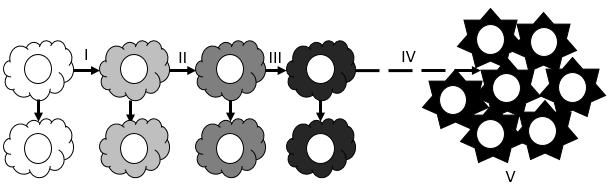
\includegraphics{img/fig-evolution.png}}
\end{center}\vspace*{-0.6cm}
\caption[Proceso de acumulaci\'on de mutaciones que provocan la aparici\'on del c\'ancer]{Proceso de acumulaci\'on de mutaciones que provocan la aparici\'on del c\'ancer~\cite{robins}. Las mutaciones sufridas por las poblaciones de c\'elulas y sus descendientes son las siguientes: aparece una mutaci\'on inicial que desactiva un inhibidor del ciclo celular~(\emph{I}); la c\'elula mutada contin\'ua su divisi\'on y un descendiente adquiere una nueva mutaci\'on que activa un estimulante del ciclo celular~(\emph{II}); el proceso contin\'ua y aparece una c\'elula con una nueva mutaci\'on que desactiva un factor de estabilidad gen\'omico~(\emph{III}); las mutaciones se acumulan r\'apidamente por la p\'erdida de la estabilidad gen\'etica hasta que aparece la primera c\'elula cancer\'igena~(\emph{IV}); aparece el c\'ancer como enfermedad por la divisi\'on descontrolada de estas c\'elulas altamente mutadas~(\emph{V}).}
\label{fig-evolution}
\end{figure}

\section{Inmortalidad replicativa}
\label{subsec-inm-rep}
Todos los organismos tienen formas y tama\~nos definidos, tanto a nivel celular como a nivel de tejidos. Casi todos los tipos de c\'elulas del organismo poseen un conjunto de se\~nales y mecanismos que controlan su ritmo de proliferaci\'on. Este control es vital para mantener la integridad de las c\'elulas y el tejido. Si las c\'elulas se dividieran de forma descontrolada sin ning\'un tipo de restricci\'on, los tejidos podr\'ian desarrollarse hasta alcanzar tama\~nos enormes con resultados letales para el organismo~\cite{hanahan}.

Las c\'elulas cancer\'igenas se definen t\'ipicamente por su capacidad de dividirse sin control alguno. Para que un peque\~no conjunto de c\'elulas clonales se expandan hasta el tama\~no de un tumor potencialmente fatal debe existir un trastorno en los mecanismos celulares que controlan su divisi\'on. En un cultivo las c\'elulas normales pueden llevar a cabo una cantidad finita de divisiones antes de que detengan su divisi\'on completamente, mientras que las c\'elulas cancer\'igenas pueden dividirse indefinidamente. Esto ocurre porque las c\'elulas poseen un n\'umero finito de posibles divisiones celulares o potencial replicativo. Una c\'elula humana puede dividirse de 60 a 70 veces como promedio antes de que incurra en un proceso conocido como senescencia. Una c\'elula senescente es viable pero ha perdido su capacidad de dividirse. Un ejemplo de la inmortalidad replicativa de las c\'elulas cancer\'igenas son las c\'elulas HeLa. Estas c\'elulas fueron cultivadas de un adenocarcinoma cervical de un paciente de c\'ancer llamado Henrietta Lacks en 1951, y hasta el d\'ia de hoy estas c\'elulas contin\'uan su crecimiento y proliferaci\'on en cientos de laboratorios alrededor del mundo. Esto sugiere claramente que estas c\'elulas cancer\'igenas han interrumpido los mecanismos de senescencia en el interior de la c\'elula ganando un potencial replicativo ilimitado~\cite{robins,hanahan,cancerbook}.

El mecanismo que se encarga de la senescencia es un contador que controla la cantidad finita de divisiones celulares y se encuentra en los extremos de todos los cromosomas del cuerpo humano: los tel\'omeros. Los tel\'omeros son secuencias de material gen\'etico que no codifican ninguna prote\'ina por lo que se conoce como secuencias basura. No obstante, juegan un papel fundamental en la protecci\'on de los cromosomas. Su importancia radica en un problema \'unico presente en la replicaci\'on del c\'odigo gen\'etico durante la divisi\'on celular. Despu\'es de cada ronda de replicaci\'on del c\'odigo gen\'etico se pierde una corta secuencia del tel\'omero en los extremos de cada cromosoma. Como resultado de la degradaci\'on de los tel\'omeros los cromosomas se hacen m\'as cortos. Los ciclos sucesivos de replicaci\'on traen como consecuencia una erosi\'on continua de los tel\'omeros hasta el punto en que comienzan a causar problemas en el c\'odigo gen\'etico tales como cambios gen\'eticos, errores de escritura y muerte celular. Por tanto, una c\'elula normal posee un ciclo vital finito, dictado por la longitud de sus tel\'omeros~(Fig.\ref{fig-telomero})~\cite{robins,hanahan,cancerbook}.

\begin{figure}[!ht]
\begin{center}
\scalebox{0.75}{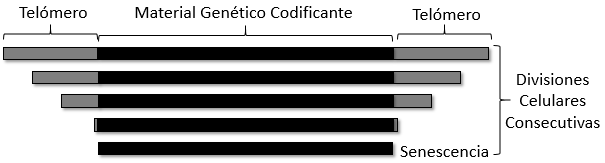
\includegraphics{img/fig-telomero.png}}
\end{center}\vspace*{-0.6cm}
\caption[Proceso de degradaci\'on de los tel\'omeros de una c\'elula]{Proceso de degradaci\'on de los tel\'omeros de una c\'elula a medida que ocurren divisiones celulares consecutivas hasta alcanzar el estado de senescencia.}
\label{fig-telomero}
\end{figure}

Las c\'elulas cancer\'igenas por otra parte, mantienen la longitud de sus te\-l\'omeros sin la p\'erdida de material gen\'etico codificante. La principal estrategia utilizada para mantener la longitud de los tel\'omeros es mediante la activaci\'on de una enzima llamada telomerasa. El $85$-$90\%$ de todas las formas de c\'ancer presentan la activaci\'on de telomerasa. La telomerasa mantiene la longitud de los tel\'omeros por encima del umbral cr\'itico, previniendo la erosi\'on y habilitando un potencial replicativo ilimitado~\cite{robins,hanahan,cancerbook}.

La evidencia listada sugiere que la senescencia es un mecanismo de protecci\'on utilizado por las c\'elulas para entrar en una fase inactiva que detiene su proliferaci\'on. Los tumores evitan la senescencia activando la telomerasa por lo que las estrategias terap\'euticas encaminadas a inhibir la telomerasa afectar\'a preferentemente a c\'elulas cancer\'igenas y no al correcto funcionamiento del organismo. 

\section{Oncogenes}
\label{subsec-oncogene}
Las c\'elulas no pueden sobrevivir en aislamiento. Las c\'elulas forman parte de un tejido o \'organo y su comportamiento casi siempre depende de se\~nales de crecimiento provenientes del entorno que activan la divisi\'on celular. Estas se\~nales de crecimiento se adhieren a la c\'elula y promueven o inhiben la expresi\'on de genes espec\'ificos. Entre las se\~nales de crecimiento est\'an los factores de crecimiento, las prote\'inas de la matriz extracelular~(de ahora en adelante ECM) y las mol\'eculas de adhesi\'on e interacci\'on intercelular. Si estas se\~nales est\'an ausentes una c\'elula normal entrar\'ia en un estado inactivo y no llevar\'ia a cabo divisiones celulares activas. Esta dependencia de se\~nales de crecimiento externas es un mecanismo cr\'itico para controlar el comportamiento de las c\'elulas que conforman un tejido~\cite{robins,hanahan,cancerbook}. 

Las c\'elulas cancer\'igenas por otra parte, generan prote\'inas mutantes~(prote\'inas oncog\'enicas) que imitan las se\~nales de crecimiento normales~(prote\'inas protooncog\'enicas). La transformaci\'on de protooncogenes en oncogenes puede ser el resultado de numerosos factores como mutaciones, reorganizaciones cromos\'omicas, amplificaciones de genes entre otras. La consecuencia de la transformaci\'on oncog\'enica es que las c\'elulas del tumor se vuelven independientes de estas se\~nales externas de crecimiento. Esta habilidad adquirida por las c\'elulas tumorales puede ser demostrada de forma emp\'irica en cultivos \textit{in vitro}~\cite{robins,hanahan,cancerbook}.

Las c\'elulas normales que han sido cultivadas \textit{in vitro} no se dividen y no proliferan en ausencia de factores de crecimiento en el medio de cultivo. Las c\'elulas tumorales en cambio pueden proliferar activamente sin depender de estos factores. Pueden adem\'as crear sus propios factores mediante mutaciones en los mecanismos de fabricaci\'on haciendo que est\'en siempre activas e ignoren las se\~nales que interrumpen su funcionamiento. En \'ultima instancia pueden inducir la producci\'on de estos factores en las c\'elulas vecinas sanas para suplir su demanda~(Fig.\ref{fig-growth-factor}). Esta autonom\'ia de los factores de crecimiento conlleva a una proliferaci\'on descontrolada e incrementa las probabilidades de adquirir nuevas mutaciones en el c\'odigo gen\'etico~\cite{robins,hanahan,cancerbook}.

\begin{figure}[!ht]
\begin{center}
\scalebox{0.65}{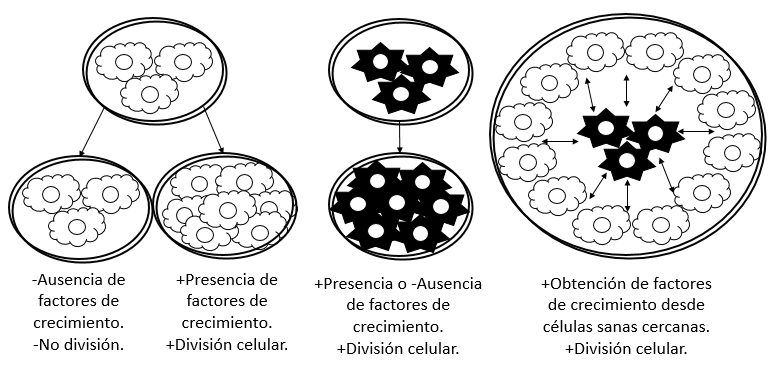
\includegraphics{img/fig-growth-factor.png}}
\end{center}\vspace*{-0.6cm}
\caption[Representaci\'on de las distintas mutaciones que sufren las c\'elulas cancer\'igenas que modifican su respuesta ante la presencia o no de factores de crecimiento, en comparaci\'on con las c\'elulas sanas]{Representaci\'on de las distintas mutaciones que sufren las c\'elulas cancer\'igenas que modifican su respuesta ante la presencia o no de factores de crecimiento, en comparaci\'on con las c\'elulas sanas~\cite{robins}.}
\label{fig-growth-factor}
\end{figure}

\section{Genes supresores de tumores}
\label{subsec-supp-genes}
El balance entre la proliferaci\'on y la inactividad celular es el resultado de una compleja interacci\'on entre los reguladores del ciclo celular: los estimulantes y los inhibidores. Como apreciamos anteriormente, los estimulantes comprenden una variedad de se\~nales y factores de crecimiento que activan la proliferaci\'on celular. Sin embargo, los tejidos sanos tambi\'en est\'an sujetos a se\~nales antiproliferaci\'on que son responsables de la inactividad celular, y act\'uan como frenos a las se\~nales de crecimiento. Los inhibidores pueden estar presentes en la ECM y en la superficie celular~\cite{robins,hanahan,cancerbook}. 

De forma similar a las se\~nales de crecimiento, las se\~nales que bloquean o suprimen la divisi\'on celular se reciben a trav\'es de receptores en la superficie de la c\'elula y promueven o inhiben la expresi\'on de genes espec\'ificos. Los genes que codifican esta clase de prote\'inas involucradas en la supresi\'on de la divisi\'on celular se conocen como genes supresores de tumores. Las c\'elulas normales, antes de la divisi\'on celular, verifican constantemente su medio interno y externo para asegurarse de que las condiciones son ideales para la mitosis~(reparto equitativo del material hereditario caracter\'istico). Las se\~nales provenientes del medio externo o interno dictan si la c\'elula deber\'ia dividirse, volverse inactiva o destruirse. Este mecanismo constituye una forma de mantener la homeostasis en el organismo, asegur\'andose que las c\'elulas se dividan en el momento justo y bajo condiciones \'optimas~\cite{robins,hanahan,cancerbook}.

Las c\'elulas cancer\'igenas por otra parte desv\'ian o evaden estas se\~nales de no proliferaci\'on para habilitar su propio crecimiento. Por ejemplo, las mutaciones en los genes que codifican inhibidores del ciclo celular podr\'ian resultar en una divisi\'on celular incrementada. Los genes supresores de tumores constituyen un grupo grande de genes que codifican prote\'inas cuyo rol fundamental es la restricci\'on del ciclo celular. Las mutaciones en estos genes pueden traer como consecuencia una p\'erdida de funcionalidad~\cite{robins,hanahan,cancerbook}.

\section{Apoptosis}
\label{subsec-apopt}
Las c\'elulas verifican constantemente su estado interno incluyendo su acceso a nutrientes y ox\'igeno, la integridad de su genoma y el balance entre los reguladores del ciclo celular. Si esta revisi\'on detecta alg\'un da\~no o mal funcionamiento, se activan sistemas de respaldo que determina si la c\'elula deber\'ia interrumpir su proliferaci\'on y llevar a cabo labores de reparaci\'on o si el da\~no es severo si deber\'ia llevar a cabo la muerte celular. El desarrollo de tumores puede ser visto no como una simple proliferaci\'on excesiva, sino tambi\'en como una reducci\'on en las muertes celulares. La muerte celular programada o apoptosis representa una parte importante en esta hip\'otesis. Existe evidencia en aumento que sugiere que la evasi\'on o resistencia a la apoptosis es una caracter\'istica distintiva de casi todas las formas de c\'ancer~\cite{robins,hanahan,cancerbook}.

La muerte celular programada es parte del desarrollo y crecimiento normales. La homeostasis del tejido es un balance entre las divisiones y muertes celulares, donde la cantidad de c\'elulas que conforman el tejido se mantiene relativamente constante. Si este equilibrio se perturba puede llevar a que las c\'elulas se dividan m\'as r\'apido de lo que mueren, resultando en el desarrollo del c\'ancer o mueran m\'as r\'apido de lo que pueden dividirse, resultando en una atrofia del tejido. La desregulaci\'on de esta compleja homeostasis del tejido se encuentra implicada en muchas formas de c\'ancer.

Las se\~nales de apoptosis pueden provenir del interior de la c\'elula como del medio externo, y activan la muerte celular de forma muy precisa y coordinada. Los principales componentes de estas se\~nales pueden dividirse en dos partes: la primera es la detecci\'on de la se\~nal de apoptosis y la segunda es la ejecuci\'on de la se\~nal. La c\'elula verifica los medios interno y externo para detectar cambios en las condiciones del entorno que puedan influir en su ciclo celular. Entre las se\~nales del medio externo que pueden causar la apoptosis se encuentran la exposici\'on a toxinas y a ciertas hormonas. Las se\~nales internas dependen de si existe o no da\~no en el material gen\'etico o la c\'elula est\'a sujeta a condiciones de estr\'es que pueden afectarla f\'isicamente. Entre estos factores internos se encuentran el calor, la radiaci\'on, la falta de ox\'igeno, la insuficiencia de factores de crecimiento, infecciones virales o un incremento del calcio en el interior de la c\'elula. Es aceptado actualmente que sin importar el origen de la se\~nal, ambas activan mecanismos comunes encargados de llevar a cabo la muerte celular programada~\cite{robins,hanahan,cancerbook}.

Las c\'elulas cancer\'igenas pueden afectar los mecanismos de la apoptosis de muchas maneras, pero el m\'etodo m\'as com\'un involucra mutaciones del gen supresor de tumores \textit{p53}. La funci\'on principal del gen \textit{p53} es la de detectar da\~nos en el c\'odigo gen\'etico y determinar el curso de acci\'on. Si el da\~no es reparable el gen \textit{p53} induce labores de reparaci\'on en el c\'odigo gen\'etico, pero si el da\~no es irreparable, entonces es el encargado de enviar una se\~nal para llevar a cabo la apoptosis. M\'as del $50\%$ de todas las formas de c\'ancer del ser humano y el $80\%$ de los carcinomas de c\'elulas escamosas muestran una inactivaci\'on de este gen~(Fig.\ref{fig-apoptosis}). Este es el ejemplo m\'as com\'un, pero en la c\'elula existen una mayor cantidad de mecanismos de detecci\'on de se\~nales de muerte celular y ejecuci\'on de dicha se\~nal. Es improbable que una forma dada de c\'ancer haya perdido todos los mecanismos relacionados con la apoptosis. La identificaci\'on de los mecanismos que retienen su funcionalidad constituye una v\'ia de combatir la enfermedad mediante el dise\~no de drogas que tengan como objetivo su activaci\'on~\cite{robins,hanahan,cancerbook}.

\begin{figure}[!ht]
\begin{center}
\scalebox{0.65}{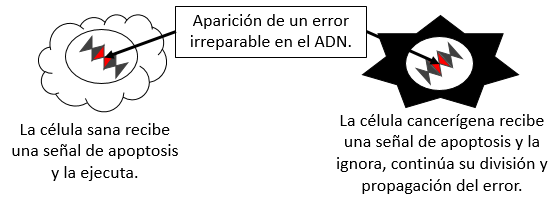
\includegraphics{img/fig-apoptosis.png}}
\end{center}\vspace*{-0.6cm}
\caption[Representaci\'on del proceso de apoptosis en una c\'elula sana y una cancer\'igena ante la aparici\'on de un error en el c\'odigo gen\'etico]{Representaci\'on del proceso de apoptosis en una c\'elula sana y una cancer\'igena ante la aparici\'on de un error en el c\'odigo gen\'etico~\cite{robins}.}
\label{fig-apoptosis}
\end{figure}

Es evidente que los cambios en los mecanismos que llevan a cabo la apoptosis pueden afectar dram\'aticamente la din\'amica de la progresi\'on tumoral, haciendo de estos cambios un factor clave para el desarrollo del c\'ancer. 

\section{Angiog\'enesis}
\label{subsec-angio}
Las c\'elulas y los tejidos necesitan ox\'igeno y nutrientes para sobrevivir y proliferar por lo que la mayor\'ia de las c\'elulas yacen a menos de $0$.$1mm$ de un capilar sangu\'ineo. Bajo la mayor\'ia de las circunstancias las c\'elulas que conforman el endotelio, tejido que recubre la zona interna de todos los vasos sangu\'ineos y el coraz\'on, no se dividen ni crecen. Sin embargo, bajo ciertas situaciones como la sanaci\'on de una herida, se activa la divisi\'on de las c\'elulas endoteliales provocando el crecimiento de nuevos capilares sangu\'ineos. Este proceso se conoce como angiog\'enesis o neovascularizaci\'on.

Los tumores tienen la capacidad de inducir la angiog\'enesis y constituye un paso fundamental en la transici\'on de un grupo peque\~no de c\'elulas mutadas~(tumor \textit{in situ}) en un crecimiento maligno capaz de invadir los tejidos vecinos y \'organos distantes. Esta transici\'on puede tomar muchos meses o a\~nos, y a menos que se induzca la angiog\'enesis, los tumores s\'olidos no crecer\'an m\'as de $1$-$2mm$. Como ocurre con la mayor\'ia de los mecanismos que mantienen la homeostasis celular, la angiog\'enesis tambi\'en comprende un balance entre se\~nales positivas y negativas que estimulan o inhiben este proceso. Se conoce que la habilidad para inducir y mantener la angiog\'enesis se adquiere en una serie de pasos discretos durante el desarrollo tumoral. Se muestra a continuaci\'on una revisi\'on simplificada de este proceso~\cite{robins,hanahan,cancerbook}:

\begin{enumerate}
\item [I.] El tumor libera factores angiog\'enicos que se difunden en los tejidos cercanos y se acoplan a receptores en las c\'elulas endoteliales de los vasos sangu\'ineos preexistentes, provocando su activaci\'on.

\item [II.] Tales interacciones entre las c\'elulas tumorales y las endoteliales conlleva a la secreci\'on y activaci\'on de enzimas que degradan la membrana basal y la matriz extracelular.

\item [III.] La degradaci\'on de la membrana basal permite que las c\'elulas endoteliales activas migren hacia el tumor.

\item [IV.] Las c\'elulas endoteliales depositan una nueva membrana basal y secretan factores de crecimiento que atraen a c\'elulas de soporte de la matriz extracelular para que estabilicen el nuevo vaso sangu\'ineo.
\end{enumerate}

Sin embargo, todav\'ia no se comprenden por completo los mecanismos que afectan el balance angiog\'enico a favor del tumor. El escenario m\'as probable es que existan relaciones entre estos mecanismos de balance y otros reguladores de la homeostasis celular. Por ejemplo, el gen supresor de tumores \textit{p53} se encuentra estrechamente relacionado con un inhibidor angiog\'enico. Por tanto, cualquier afectaci\'on al normal funcionamiento del gen \textit{p53}, que es com\'un en el desarrollo tumoral, puede causar una ca\'ida en los niveles del inhibidor provocando un desbalance angiog\'enico~\cite{robins,hanahan,cancerbook}.

La angiog\'enesis tumoral constituye un blanco irresistible para el desarrollo de terapias que afecten el desarrollo tumoral. En la actualidad los tratamientos antiangiog\'enicos constituyen una fracci\'on numerosa de los ensayos cl\'inicos que se est\'an llevando a cabo para combatir el c\'ancer.

\section{Met\'astasis}
\label{subsec-meta}
Los tumores s\'olidos, bajo condiciones \'optimas, pueden invadir los tejidos locales y atravesar el sistema circulatorio para colonizar \'organos y tejidos distantes. Estos tumores secundarios son responsables de casi el $90\%$ de las muertes relacionadas con el c\'ancer. La capacidad de las c\'elulas tumorales de invadir y colonizar es la sexta marca distintiva del c\'ancer. Seg\'un~\cite{robins,hanahan}, las definiciones de los t\'erminos \textit{invasi\'on local} y \textit{met\'astasis} son:

\paragraph{Invasi\'on local:}El crecimiento del c\'ancer se acompa\~na de una infiltraci\'on, invasi\'on y destrucci\'on progresivas del tejido circundante, mostrando un rompimiento de la membrana basal. Adem\'as de las met\'astasis, la capacidad de invasi\'on es el rasgo m\'as fiable para distinguir el c\'ancer de los tumores benignos.

\paragraph{Met\'astasis:}Se define como la propagaci\'on del tumor a sitios f\'isicamente alejados del tumor primario y marca, de un modo inequ\'ivoco, dicho tumor como maligno ya que por definici\'on, una neoplasia benigna no metastatiza.\vspace*{0.5cm}

Una vez que un tumor infiltra satisfactoriamente los tejidos vecinos sanos, las c\'elulas cancer\'igenas que lo conforman sufren distintas transformaciones que provocan la p\'erdida de la capacidad de adhesi\'on celular y cambios en la matriz de interacci\'on intercelular~\cite{hanahan,invasion}. La disminuci\'on de la adhesi\'on celular permite que ocurran desprendimientos de c\'elulas cancer\'igenas pertenecientes al tumor primario. Estas c\'elulas sufren cambios en la matriz de interacci\'on celular que provocan la expresi\'on de prote\'inas involucradas en el control de la movilidad, la supresi\'on de reguladores de la migraci\'on y la degradaci\'on de la ECM y la membrana basal. De esta forma pueden migrar a trav\'es del tejido circundante y adaptarse r\'apidamente para vencer numerosas dificultades que presentan los nuevos entornos~\cite{hanahan,invasion}. Estas c\'elulas tambi\'en son la causa fundamental de las recurrencias cuando la masa principal del tumor es removida quir\'urgicamente~\cite{kansal3}. 

Las c\'elulas cancer\'igenas muestran una variedad de estrategias de migraci\'on y pueden alternar entre ellas para hacerle frente a entornos hostiles~\cite{migration}. Los factores determinantes en el proceso de migraci\'on son la expresi\'on de mecanismos de uni\'on intercelulares y los cambios de la estructura de las c\'elulas invasivas. La invasi\'on individual puede ser llevada a cabo por c\'elulas con estructuras espigadas, elongadas y redondeadas~\cite{migration} que degradan la matriz extracelular y se mueven a trav\'es de ella. La invasi\'on colectiva puede darse en forma de conjuntos migrantes que se desprenden del tumor o formando largas cadenas invasivas que parten desde el mismo~\cite{robins,hanahan,cancerbook}.

Eventualmente las c\'elulas migrantes entran en contacto con el sistema circulatorio, ya sea con capilares sangu\'ineos o vasos linf\'aticos. En este punto pueden penetrar dicho sistema, viajar en su interior hasta encontrar una localizaci\'on favorable para abandonarlo y colonizar el tejido circundante. A este proceso se le conoce como met\'astasis y los pasos que la comprenden constituyen la cascada metast\'asica: invasi\'on local, migraci\'on, penetraci\'on del sistema circulatorio~(\textit{intravasation}), transporte, abandono del sistema circulatorio~(\textit{extravasation}), formaci\'on de micromet\'astasis y colonizaci\'on~\cite{robins,invasion,hanahan,cancerbook}. Una vez el tumor primario ha comenzado el proceso de angiog\'enesis, si bien las c\'elulas cancer\'igenas deben tener las caracter\'isticas necesarias para efectuar la invasi\'on local, pueden acceder al sistema circulatorio desde los reci\'en formados capilares sangu\'ineos que sustentan al tumor, sin la necesidad de penetrar los tejidos vecinos.

Las mutaciones necesarias para que las c\'elulas cancer\'igenas sean capaces de efectuar la invasi\'on local y la met\'astasis son comunes para ambos procesos. Sin embargo, para la colonizaci\'on satisfactoria de un \'organo distante estas c\'elulas deben poseer una mayor resistencia. El proceso de met\'astasis es altamente ineficiente~\cite{pubmed}, ya que la cantidad de c\'elulas que dejan el tumor primario son del orden de los millones en un d\'ia, pero solo una peque\~na fracci\'on de las mismas son capaces de sobrevivir a la cascada metast\'asica. Las c\'elulas migratorias pueden terminar su existencia por una gran variedad de causas, entre las que se encuentran:

\begin{itemize}
\item Una c\'elula sobrevive normalmente conectada a sus vecinos y al conjunto de prote\'inas existente a su alrededor. El desprendimiento de la superficie de otras c\'elulas puede llevar a la muerte celular.
\item Las c\'elulas cancer\'igenas son con frecuencia mucho mayores en tama\~no que las c\'elulas que viven en el sistema circulatorio. Cuando estas viajan a trav\'es de dicho sistema pueden da\~narse o atascarse, llevando a la muerte celular.
\item Las c\'elulas cancer\'igenas pueden ser reconocidas y destruidas por c\'elulas del sistema inmunitario.
\end{itemize}

A\'un cuando una c\'elula metast\'asica sobrevive todo el proceso, esto no significa que forme un tumor secundario satisfactoriamente. Dicha c\'elula debe crear un entorno favorable dentro de un nuevo ambiente hostil que les permita sobrevivir y crecer. Esta capacidad de transformar el entorno es un hecho crucial como lo demuestran numerosos experimentos~\cite{pubmed}. En un estudio experimental de un melanoma metast\'asico, m\'as del $80\%$ de las c\'elulas cancer\'igenas sobrevivieron al transporte a trav\'es del sistema circulatorio y arribaron al h\'igado. De estas, solamente $1$ c\'elula de cada $40$ formaron micromet\'astasis en un lapso de $3$ d\'ias, y $1$ de cada $100$ formaron macromet\'astasis en $10$ d\'ias. La tarea de crear un entorno favorable parece ser un proceso complejo que limita notablemente la capacidad de la c\'elula de formar un tumor secundario. Cuando una c\'elula cancer\'igena entra en contacto con un nuevo \'organo, puede ocurrir una de tres variantes:

\begin{itemize}
\item El tejido circundante del nuevo \'organo puede ser muy diferente de donde se origin\'o el tumor primario, y en la mayor\'ia de los casos puede ser muy hostil, al punto de impedir la supervivencia de la c\'elula cancer\'igena, llevando a su muerte celular. 
\item Si dicha c\'elula metast\'asica no posee la capacidad de transformar el tejido en un entorno m\'as amistoso, no podr\'a colonizar satisfactoriamente. En este caso se dice que la c\'elula entra en un per\'iodo de dormancia, no muere, pero no es capaz de crecer. Ocasionalmente dichas micromet\'astasis latentes obtienen nuevas mutaciones que les permite colonizar satisfactoriamente dicho \'organo.
\item La c\'elula migrante posee todas las capacidades necesarias para colonizar la nueva localizaci\'on, como se ha comprobado en tumores que hacen met\'astasis en el mismo \'organo donde surgi\'o el tumor primario, o en \'organos espec\'ificos. Distintos tipos de c\'ancer tienen preferencia por \'organos espec\'ificos para ser atacados por c\'elulas migratorias~\cite{invasion}.
\end{itemize}

Precisamente la tendencia de colonizar \'organos espec\'ificos seg\'un los diferentes tipos de c\'ancer se conoce como la hip\'otesis de la semilla y el sustrato~(\textit{the seed and soil hypothesis})~\cite{paget}. En 1889 Stephen Paget observ\'o que los pacientes con c\'ancer de mama desarrollaban tumores secundarios en el h\'igado con frecuencia. Consider\'o que era poco probable que esto sucediese principalmente por la accesibilidad del h\'igado al sistema circulatorio, ya que otros \'organos que poseen un acceso al suministro de sangre equivalente desarrollaban met\'astasis muy rara vez. En base a esto, desarroll\'o dicha hip\'otesis, en la cual ciertas c\'elulas cancer\'igenas solo pueden colonizar satisfactoriamente \'organos selectos que poseen entornos de crecimiento adecuados o deseables~\cite{paget,metastasis}, entre los que se incluye el entorno del \'organo primario. Esta hip\'otesis comprende tres conceptos importantes:

\begin{itemize}
\item Los tumores primarios y sus met\'astasis est\'an compuestos de c\'elulas tumorales gen\'eticamente muy diversas.
\item Las c\'elulas seleccionadas para llevar a cabo la met\'astasis son las que pueden sobrevivir a toda la cascada.
\item Las c\'elulas seleccionadas colonizan una localizaci\'on en una forma muy espec\'ifica, y dado que los entornos de cada \'organo son distintos las c\'elulas cancer\'igenas solo podr\'an colonizar un tipo de \'organo espec\'ifico.
\end{itemize}

Estos conceptos muestran la idea de que una met\'astasis satisfactoria depende completamente de las interacciones entre las c\'elulas cancer\'igenas y las c\'elulas del \'organo objetivo. Estas c\'elulas que reci\'en est\'an formando una nueva met\'astasis no solo tienen que ser capaces de producir los factores requeridos por ellas para sobrevivir y crecer en el nuevo entorno, sino que el entorno del nuevo \'organo tiene que ser capaz de responder a estas se\~nales y actuar en consecuencia. Si la c\'elula cancer\'igena se encuentra en un entorno muy inh\'ospito ser\'a imposible que una met\'astasis se forme satisfactoriamente~\cite{metastasis}. Si una c\'elula cancer\'igena sobrevive al transporte en el interior del sistema circulatorio y lleva a cabo la extravasaci\'on de forma satisfactoria puede ocurrir una de tres situaciones~\cite{circulating}:

\begin{itemize}
\item La extravasaci\'on de la c\'elula ocurre en la localizaci\'on del tumor donde se origin\'o, es decir, penetr\'o el sistema circulatorio, sobrevivi\'o a su transporte y arrib\'o al propio punto de origen. En este caso contribuye a la poblaci\'on tumoral en la localizaci\'on primaria.
\item La extravasaci\'on de la c\'elula ocurre en la localizaci\'on de una met\'astasis. En este caso se comporta de igual forma, contribuyendo con la poblaci\'on tumoral.
\item La extravasaci\'on de la c\'elula ocurre en una localizaci\'on no colonizada a\'un. En este caso puede asentarse y comenzar una nueva met\'astasis.
\end{itemize}

\section{Evoluci\'on macrosc\'opica del c\'ancer}
\label{subsec-macro}
La c\'elula cancer\'igena a medida que acumula mutaciones adquiere nuevas capacidades que alteran el comportamiento del tumor. La obtenci\'on de las seis mutaciones distintivas provocan los cambios m\'as evidentes y proveen de un modelo ideal para describir su progresi\'on macrosc\'opica y las transiciones entre las distintas etapas. Para ilustrar este proceso se utiliza como referencia el grupo de neoplasias conocidas como carcinomas que representan el $80\%$ de los tumores malignos. Estos tienen su origen en el epitelio, tejido que recubre gran parte del organismo como el revestimiento interno de las cavidades, \'organos huecos, conductos, mucosas, gl\'andulas y en muchos casos constituyen el tejido funcional. Se trata de capas de c\'elulas fuertemente enlazadas que descansan sobre una membrana basal, separ\'andolas del tejido de sost\'en subyacente. El epitelio carece de vasos sangu\'ineos por lo que su sustento depende de la difusi\'on de nutrientes a trav\'es de la membrana basal provenientes de los capilares sangu\'ineos presentes en el tejido de sost\'en~(Fig.\ref{fig-epitelium}).

\begin{figure}[!ht]
\begin{center}
\scalebox{0.75}{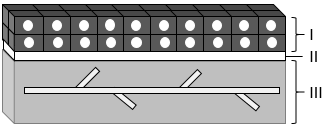
\includegraphics{img/fig-epitelium.png}}
\end{center}\vspace*{-0.6cm}
\caption[Distribuci\'on del tejido epitelial, la membrana basal y el tejido de sost\'en subyacente]{Distribuci\'on del tejido epitelial~(I), la membrana basal~(II) y el tejido de sost\'en subyacente~(III). Se observa la vasculatura del tejido de sost\'en.}
\label{fig-epitelium}
\end{figure}

El desarrollo de una neoplasia maligna se divide en dos etapas principales: la etapa celular y la etapa macrosc\'opica. La primera se refiere a la evoluci\'on temprana del tumor, cuando las c\'elulas proliferantes no han comenzado a aglomerarse. La segunda comienza cuando agrupaciones de estas c\'elulas proliferantes se condensan en una forma compacta. El cambio m\'as notable durante la evoluci\'on macrosc\'opica es el relacionado con el proceso de angiog\'enesis que hace que el tumor aumente r\'apida y considerablemente de tama\~no. Por este hecho se usa la vascularizaci\'on como l\'inea divisoria entre las etapas macrosc\'opicas~\cite{vascular}. 

La etapa avascular se caracteriza por un desarrollo local de la neoplasia, con un rango de acci\'on y peligrosidad limitadas, en el que las c\'elulas tumorales presentan un alto grado de adhesi\'on, haciendo del tumor una masa compacta con forma semiesf\'erica~\cite{ruben,vascular}. La difusi\'on de los nutrientes y el ox\'igeno transportados por el sistema circulatorio constituye la forma de sustento principal del tumor. En diversos estudios \textit{in vitro} se han utilizado MTS para simular el desarrollo avascular tumoral. Estos exhiben una proliferaci\'on exponencial inicial seguida de una saturaci\'on en el crecimiento, incluso en presencia de un suministro constante de nutrientes. Los procesos responsables de este comportamiento se relacionan con la auto organizaci\'on de las c\'elulas tumorales y el alcance limitado de la difusi\'on~\cite{kansal,dormann}. Se puede inferir que sin una nueva forma de obtener los nutrientes el tumor no puede crecer por encima de $1$ o $2mm$. Durante esta etapa las c\'elulas cancer\'igenas presentan en alguna medida las mutaciones distintivas relacionadas directamente con el ciclo celular: la inmortalidad replicativa, la producci\'on de se\~nales de crecimiento, la evasi\'on de se\~nales que inhiben su proliferaci\'on y la resistencia a la muerte celular. A medida que progresa esta etapa, dichas mutaciones se vuelven m\'as marcadas aumentando la malignidad del tumor~\cite{vascular}. A pesar de esto, rara vez muestran signos de invasi\'on local, confin\'andose al tejido donde se origin\'o la neoplasia, lo que se conoce como tumor \textit{in situ}~(Fig.\ref{fig-epitelium-2}).

\begin{figure}[!ht]
\begin{center}
\scalebox{0.5}{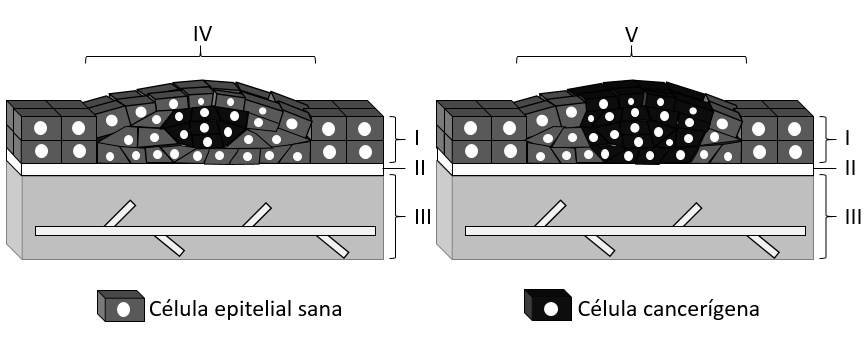
\includegraphics{img/fig-epitelium-2-horizontal.png}}
\end{center}\vspace*{-1cm}
\caption[Evoluci\'on de un tumor durante la etapa avascular]{Evoluci\'on de un tumor durante la etapa avascular. Se aprecia en ambos esquemas el desplazamiento de las c\'elulas sanas del epitelio~(\emph{I}) por la expansi\'on del tumor~(\emph{IV}, \emph{V}). Eventualmente la lesi\'on se vuelve visible en la cavidad~(\emph{V}) pues las c\'elulas cancer\'igenas se alzan sobre el epitelio. La membrana basal~(\emph{II}) se mantiene intacta y no existe invasi\'on del tejido de sost\'en subyacente~(\emph{III}) por parte del tumor.}
\label{fig-epitelium-2}
\end{figure}

\begin{figure}[!ht]
\begin{center}
\scalebox{0.5}{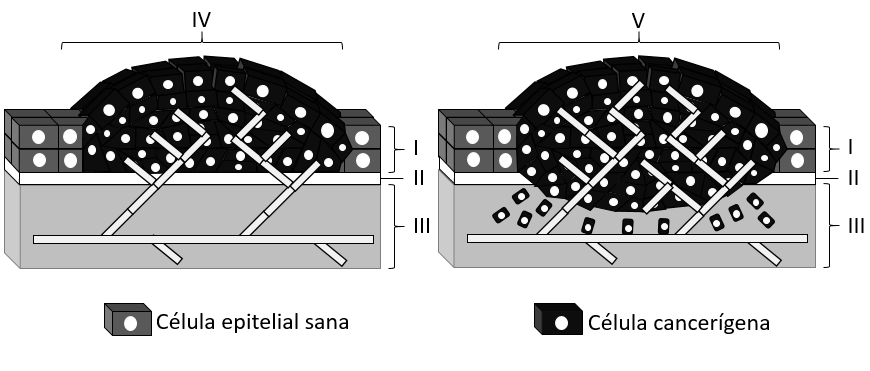
\includegraphics{img/fig-epitelium-3-horizontal.png}}
\end{center}\vspace*{-1cm}
\caption[Evoluci\'on de un tumor durante la etapa vascular]{Evoluci\'on de un tumor durante la etapa vascular. Se aprecia en ambos esquemas el incremento de la neovasculatura inducida por el tumor~(\emph{IV}, \emph{V}). En un principio las c\'elulas cancer\'igenas~(\emph{IV}) no son capaces de penetrar la membrana basal~(\emph{II}). Pero el progreso de la angiog\'enesis degrada esta membrana~(\emph{II}) permitiendo la invasi\'on~(\emph{V}) del tejido de sost\'en subyacente~(\emph{III}). En los instantes de m\'aximo desarrollo de la neoplasia ocurren desprendimientos de c\'elulas que proceden a continuar la cascada metast\'asica~(\emph{V}).}
\label{fig-epitelium-3}
\end{figure}

Una vez que el tumor alcanza el m\'aximo tama\~no sostenible mediante la difusi\'on de nutrientes, comienza su entrada en la etapa vascular. El evento que define la transici\'on de una etapa a la otra es la adquisici\'on, por parte de las c\'elulas cancer\'igenas, de la capacidad de producir factores angiog\'enicos que penetran el tejido sano circundante y estimulan el crecimiento de nuevos vasos sangu\'ineos~\cite{robins,vascular}. Estos vasos reci\'en formados penetran la masa del tumor aliment\'andolo con abundantes nutrientes y potenciando su crecimiento por encima del m\'aximo permitido~\cite{vascular,invasion}. Como consecuencia del proceso de angiog\'enesis y de los cambios en la matriz de interacci\'on de las c\'elulas tumorales ocurre una degradaci\'on de la membrana basal y de la matriz extracelular. Esto posibilita la invasi\'on local de los tejidos vecinos, abandonando la condici\'on de tumor \textit{in situ} para transformarse en un tumor invasivo. Eventualmente las c\'elulas cancer\'igenas cercanas o pertenecientes a la frontera del tumor sufren de la p\'erdida de la adhesi\'on intercelular y comienzan a expresar movilidad. De esta forma pueden desprenderse y migrar a trav\'es del tejido de sost\'en hasta alcanzar un capilar o vaso sangu\'ineo, con el objetivo de continuar y culminar la cascada metast\'asica~(Fig.\ref{fig-epitelium-3}).
